\documentclass[11pt,a4paper]{article}

\usepackage[utf8]{inputenc}
\usepackage[T1]{fontenc}
\usepackage{lmodern}
\usepackage{microtype}
\usepackage{geometry}
\usepackage{setspace}
\usepackage{parskip}

\geometry{
    left=2.5cm,
    right=2.5cm,
    top=2.5cm,
    bottom=2.5cm
}
\onehalfspacing
\raggedbottom

\usepackage{graphicx}
\usepackage{float}
\usepackage{subcaption}
\graphicspath{{./}{./assets/}{./images/}}

% Placeholder bila gambar belum tersedia
\newcommand{\testimg}[1]{%
    \IfFileExists{assets/#1}{%
        \includegraphics[width=\textwidth]{assets/#1}%
    }{%
        \fbox{\parbox[c][4cm][c]{0.95\textwidth}{\centering\itshape\small (placeholder: assets/#1)}}%
    }%
}

\usepackage{tikz}
\usetikzlibrary{shapes.geometric, shapes.misc, arrows.meta, positioning, calc, automata, quotes, trees, fit, backgrounds}

\usepackage{listings}
\usepackage{xcolor}

\definecolor{codebg}{HTML}{F7F7F7}
\definecolor{codeframe}{HTML}{DDDDDD}
\definecolor{keyword}{HTML}{005FAF}
\definecolor{comment}{HTML}{6A737D}
\definecolor{string}{HTML}{D73A49}

\lstset{
    basicstyle=\ttfamily\footnotesize,
    keywordstyle=\color{keyword}\bfseries,
    commentstyle=\color{comment}\itshape,
    stringstyle=\color{string},
    numbers=left,
    numberstyle=\tiny\color{gray},
    backgroundcolor=\color{codebg},
    frame=single,
    rulecolor=\color{codeframe},
    breaklines=true,
    tabsize=4,
    showstringspaces=false,
    language=C++,
    aboveskip=1em,
    belowskip=1em
}

\usepackage{amsmath}
\usepackage{amssymb}

\usepackage{booktabs}
\usepackage{tabularx}
\usepackage{longtable}
\usepackage{etoolbox}

\usepackage{hyperref}
\hypersetup{
    colorlinks=true,
    linkcolor=black,
    urlcolor=keyword,
    citecolor=black,
    pdfauthor={Made Branenda Jordhy, Muhammad Nur Majiid, Jason Edward Salim, Athilla Zaidan Zidna Fann},
    pdftitle={Laporan Milestone 2 - Syntax Analysis - IF2224}
}

% HEADER/FOOTER
\usepackage{fancyhdr}
\pagestyle{fancy}
\fancyhf{}
\setlength{\headheight}{36pt}
\fancyhead[L]{%
    \small\textnormal{School of Electrical Engineering and Informatics}\\[-1pt]
    \small\textnormal{Institut Teknologi Bandung}%
}
\fancyhead[R]{\IfFileExists{assets/LogoITB.png}{
\includegraphics[height=1cm]{assets/LogoITB.png}}{}}
\fancyfoot[L]{\small\textnormal{IF2224 Formal Language and Automata Theory}}
\fancyfoot[R]{\small\thepage}
\renewcommand{\headrulewidth}{0.4pt}
\renewcommand{\footrulewidth}{0.2pt}

% TITLE
\title{
    \vspace{-1.5cm}
    {\Large\textsc{IF2224 Formal Language and Automata Theory}}\\[0.35cm]
    {\LARGE\textbf{Arion Compiler - Milestone 2: Syntax Analysis}}\\[0.3cm]
    \vspace{-0.3cm}
}
\author{}
\date{\today}

\begin{document}

\maketitle
\thispagestyle{empty}

\begin{figure}[H]
    \centering
    \IfFileExists{assets/foto_kelompok.png}{%
        
\includegraphics[width=0.6\textwidth]{assets/foto_kelompok.png}%
    }{%
        \vspace{4cm}
    }
\end{figure}

\vspace{1cm}
\begin{center}
    \textbf{Made Branenda Jordhy} - 13524026 \\[0.15cm]
    \textbf{Muhammad Nur Majiid} - 13524028 \\[0.15cm]
    \textbf{Jason Edward Salim} - 13524034 \\[0.15cm]
    \textbf{Athilla Zaidan Zidna Fann} - 13524068
\end{center}

\vspace{3cm}
\begin{center}
    {\large\textbf{School of Electrical Engineering and Informatics}}\\[0.1cm]
    {\large\textbf{Institut Teknologi Bandung}}\\[0.1cm]
    {\large\textbf{Semester II 2025/2026}}\\[0.1cm]
\end{center}

\newpage
\tableofcontents
\newpage

% -----------------------------------------------------------------------
\section{Theoretical Background}

\subsection{Syntax Analysis}

\textit{Syntax analysis} adalah fase kedua dalam pipeline kompilasi, yang dijalankan
setelah \textit{lexical analysis}. Komponen yang melaksanakan tahap ini disebut
\textit{parser}. Apabila lexer memproduksi barisan token sebagai representasi leksikal
program, maka parser bertugas memverifikasi bahwa urutan token tersebut membentuk
\textit{kalimat} yang sah dalam bahasa, yaitu struktur yang dapat diturunkan dari
\textit{grammar} bahasa.

Selain melakukan verifikasi, parser juga membangun representasi hierarkis yang
disebut \textit{parse tree}. Representasi ini menjadi masukan bagi tahap analisis
semantik dan code generation pada milestone berikutnya.
Tujuan parser dapat diringkas sebagai berikut.

\begin{itemize}
    \item Memastikan urutan token membentuk struktur sintaks yang valid menurut grammar.
    \item Mendeteksi dan melaporkan \textit{syntax error} ketika token tidak sesuai grammar.
    \item Membangun representasi sintaktis program yang siap dikonsumsi tahap berikutnya.
\end{itemize}

\subsection{Context-Free Grammar (CFG)}

Grammar bahasa pemrograman umumnya didefinisikan sebagai \textit{Context-Free Grammar} (CFG).

\begin{quote}
\textbf{Definisi.}
Sebuah CFG adalah 4-tupel $G = (V,\, \Sigma,\, R,\, S)$, di mana:
$V$ adalah himpunan non-terminal,
$\Sigma$ adalah himpunan terminal (token),
$R \subseteq V \times (V \cup \Sigma)^{*}$ adalah himpunan production rules,
dan $S \in V$ adalah simbol awal.
\end{quote}

Dalam konteks Arion, $\Sigma$ adalah himpunan token yang diemisikan oleh lexer
pada Milestone~1, $V$ adalah himpunan non-terminal seperti \texttt{<program>},
\texttt{<statement>}, dan \texttt{<expression>}, sedangkan $S = \texttt{<program>}$.

\subsection{Parse Tree dan AST}

\textit{Parse tree} adalah representasi lengkap dari proses derivasi suatu string
oleh CFG. Setiap node internal pada parse tree adalah non-terminal, sedangkan
setiap daun adalah terminal. Berbeda dengan \textit{Abstract Syntax Tree} (AST),
parse tree memuat seluruh simbol gramatikal termasuk separator, parentheses, dan
non-terminal antara, sedangkan AST hanya menyimpan informasi struktural yang
relevan secara semantis. Pada Milestone~2 ini, keluaran yang diminta adalah
\textbf{parse tree}, bukan AST.

\subsection{Recursive Descent Parsing}

\textit{Recursive descent parsing} adalah teknik parsing top-down di mana setiap
non-terminal $A \in V$ direpresentasikan oleh satu fungsi rekursif. Tubuh fungsi
\texttt{parseA()} mengikuti aturan produksi $A \to \alpha_1 \mid \alpha_2 \mid \dots$
secara langsung: percabangan grammar diterjemahkan menjadi percabangan kondisi
berbasis token \textit{lookahead}, sedangkan rekursi grammar diterjemahkan menjadi
rekursi pemanggilan fungsi.

Dengan \textit{single-token lookahead} (LL(1)) yang ditingkatkan dengan beberapa
\textit{multi-token lookahead} secara terbatas, parser dapat memilih cabang produksi
yang tepat tanpa \textit{backtracking}. Sifat ini menjamin kompleksitas waktu yang
linier $O(n)$ terhadap panjang barisan token.

\begin{figure}[H]
\centering
\begin{tikzpicture}[
    node distance=1cm and 1.5cm,
    on grid,
    every node/.style={font=\small},
    src/.style={rectangle, draw, fill=codebg, rounded corners=2pt, minimum width=2.6cm, minimum height=0.7cm},
    proc/.style={rectangle, draw, fill=yellow!12, minimum width=2.6cm, minimum height=0.7cm},
    output/.style={rectangle, draw, fill=keyword!10, minimum width=2.6cm, minimum height=0.7cm},
    arr/.style={-{Stealth[length=2.5mm]}, thick}
]
    \node[src]                    (src)   {\texttt{source.txt}};
    \node[proc, right=2cm of src] (lex)   {Lexer (DFA)};
    \node[src, right=2cm of lex]  (tok)   {Token Stream};
    \node[proc, below=1.4cm of tok] (par) {Parser (RD)};
    \node[output, left=2cm of par] (tree) {Parse Tree};

    \draw[arr] (src) -- (lex);
    \draw[arr] (lex) -- (tok);
    \draw[arr] (tok) -- (par);
    \draw[arr] (par) -- (tree);
\end{tikzpicture}
\caption{Pipeline kompilasi Arion: keluaran lexer (Milestone~1) menjadi masukan parser (Milestone~2).}
\label{fig:pipeline}
\end{figure}

% -----------------------------------------------------------------------
\section{Design and Implementation}

\subsection{Overview}

Komponen parser diimplementasikan dalam C++17 sebagai kelanjutan langsung dari
program Milestone~1. Antarmuka antara lexer dan parser adalah \texttt{std::vector<Token>}
yang dihasilkan oleh \texttt{Lexer::tokenize()}. Source code parser terbagi
menjadi dua berkas: \texttt{src/header/parser.hpp} mendeklarasikan struct
\texttt{ParseNode}, kelas \texttt{Parser}, serta exception \texttt{SyntaxError};
sedangkan \texttt{src/lib/parser.cpp} mengimplementasikan seluruh fungsi rekursif
serta utilitas pencetakan parse tree (\texttt{printTree}, \texttt{writeTree}).

Setiap node parse tree direpresentasikan oleh struct sederhana berikut.

\begin{lstlisting}
struct ParseNode {
    std::string label;
    std::vector<ParseNode*> children;
};
\end{lstlisting}

\noindent
\texttt{label} menyimpan nama non-terminal (mis.\ \texttt{<expression>}) atau
representasi terminal (mis.\ \texttt{ident(x)}, \texttt{becomes}). Penghapusan
parse tree dilakukan secara rekursif melalui \texttt{destroyParseTree()} untuk
menghindari kebocoran memori.

\subsection{Hard-coded Grammar}

Sesuai spesifikasi, grammar di-\textit{hardcode} di dalam program melalui satu
fungsi per non-terminal. Tabel~\ref{tab:grammar} merangkum keseluruhan production
rules yang diimplementasikan.

\renewcommand{\arraystretch}{1.05}
\footnotesize
\begin{longtable}{l p{12cm}}
\caption{Production rules grammar Arion yang di-\textit{hardcode} pada parser.}\label{tab:grammar}\\
\toprule
\textbf{Non-terminal} & \textbf{Produksi} \\
\midrule
\endfirsthead

\toprule
\textbf{Non-terminal} & \textbf{Produksi} \\
\midrule
\endhead

\texttt{<program>}                & \texttt{<program-header> <declaration-part> <compound-statement> period} \\
\texttt{<program-header>}         & \texttt{programsy ident semicolon} \\
\texttt{<declaration-part>}       & \texttt{(<const-declaration>)* (<type-declaration>)* (<var-declaration>)* (<subprogram-declaration>)*} \\
\texttt{<const-declaration>}      & \texttt{constsy (ident eql <constant> semicolon)+} \\
\texttt{<constant>}               & \texttt{charcon | string | [(plus | minus)?\ (ident | intcon | realcon)]} \\
\texttt{<type-declaration>}       & \texttt{typesy (ident eql <type> semicolon)+} \\
\texttt{<var-declaration>}        & \texttt{varsy (<identifier-list> colon <type> semicolon)+} \\
\texttt{<identifier-list>}        & \texttt{ident (comma ident)*} \\
\texttt{<type>}                   & \texttt{ident | <array-type> | <range> | <enumerated> | <record-type>} \\
\texttt{<array-type>}             & \texttt{arraysy lbrack (<range> | ident) rbrack ofsy <type>} \\
\texttt{<range>}                  & \texttt{<constant> period period <constant>} \\
\texttt{<enumerated>}             & \texttt{lparent ident (comma ident)* rparent} \\
\texttt{<record-type>}            & \texttt{recordsy <field-list> endsy} \\
\texttt{<field-list>}             & \texttt{<field-part> (semicolon <field-part>)*} \\
\texttt{<field-part>}             & \texttt{<identifier-list> colon <type>} \\
\texttt{<subprogram-declaration>} & \texttt{<procedure-declaration> | <function-declaration>} \\
\texttt{<procedure-declaration>}  & \texttt{proceduresy ident (<formal-parameter-list>)?\ semicolon <block> semicolon} \\
\texttt{<function-declaration>}   & \texttt{functionsy ident (<formal-parameter-list>)?\ colon ident semicolon <block> semicolon} \\
\texttt{<block>}                  & \texttt{<declaration-part> <compound-statement>} \\
\texttt{<formal-parameter-list>}  & \texttt{lparent <parameter-group> (semicolon <parameter-group>)* rparent} \\
\texttt{<parameter-group>}        & \texttt{<identifier-list> colon (ident | <array-type>)} \\
\texttt{<compound-statement>}     & \texttt{beginsy <statement-list> endsy} \\
\texttt{<statement-list>}         & \texttt{<statement> (semicolon <statement>)*} \\
\texttt{<statement>}              & \texttt{<assignment-statement> | <if-statement> | <case-statement> | <while-statement> | <repeat-statement> | <for-statement> | <procedure/function-call> | $\varepsilon$} \\
\texttt{<assignment-statement>}   & \texttt{<variable> becomes <expression>} \\
\texttt{<variable>}               & \texttt{ident ((lbrack <index-list> rbrack) | (period ident))*} \\
\texttt{<if-statement>}           & \texttt{ifsy <expression> thensy <statement> (elsesy <statement>)?} \\
\texttt{<case-statement>}         & \texttt{casesy <expression> ofsy <case-block> (semicolon <case-block>)* endsy} \\
\texttt{<case-block>}             & \texttt{<constant> (comma <constant>)* colon <statement>} \\
\texttt{<while-statement>}        & \texttt{whilesy <expression> dosy <statement>} \\
\texttt{<repeat-statement>}       & \texttt{repeatsy <statement-list> untilsy <expression>} \\
\texttt{<for-statement>}          & \texttt{forsy ident becomes <expression> (tosy | downtosy) <expression> dosy <statement>} \\
\texttt{<procedure/function-call>}& \texttt{ident (lparent <parameter-list> rparent)?} \\
\texttt{<parameter-list>}         & \texttt{<expression> (comma <expression>)* | $\varepsilon$} \\
\texttt{<expression>}             & \texttt{<simple-expression> (<relational-operator> <simple-expression>)?} \\
\texttt{<simple-expression>}      & \texttt{(plus | minus)?\ <term> (<additive-operator> <term>)*} \\
\texttt{<term>}                   & \texttt{<factor> (<multiplicative-operator> <factor>)*} \\
\texttt{<factor>}                 & \texttt{intcon | realcon | charcon | string | (lparent <expression> rparent) | (notsy <factor>) | <procedure/function-call> | <variable>} \\
\texttt{<relational-operator>}    & \texttt{eql | neq | gtr | geq | lss | leq} \\
\texttt{<additive-operator>}      & \texttt{plus | minus | orsy} \\
\texttt{<multiplicative-operator>}& \texttt{times | rdiv | idiv | imod | andsy} \\
\bottomrule
\end{longtable}
\renewcommand{\arraystretch}{1.15}

\subsection{Recursive Descent Architecture}

Setiap non-terminal pada Tabel~\ref{tab:grammar} dipetakan ke satu method
private \texttt{parseX()} pada kelas \texttt{Parser}. Pemanggilan dimulai dari
\texttt{parseProgram()} dan terus turun secara rekursif sesuai struktur grammar.
Diagram~\ref{fig:rd-call} menunjukkan hierarki pemanggilan utama.

\begin{figure}[H]
\centering
\resizebox{0.95\textwidth}{!}{%
\begin{tikzpicture}[
    every node/.style={font=\footnotesize, draw, rounded corners=2pt, fill=codebg, inner sep=4pt},
    level distance=1.1cm,
    edge from parent/.style={draw, -{Stealth[length=2mm]}},
    sibling distance=2.4cm,
    level 1/.style={sibling distance=4.4cm},
    level 2/.style={sibling distance=2.6cm},
    level 3/.style={sibling distance=2cm}
]
\node {parseProgram}
    child {node {parseHeader}}
    child {node {parseDeclaration}
        child {node {parseConsts}}
        child {node {parseTypes}}
        child {node {parseVars}}
        child {node {parseSub}
            child {node {parseProc}}
            child {node {parseFunc}}
        }
    }
    child {node {parseCompound}
        child {node {parseStmtList}
            child {node {parseStmt}
                child {node {parseAssign}}
                child {node {parseIf}}
                child {node {parseCall}}
            }
        }
    };
\end{tikzpicture}}
\caption{Hierarki pemanggilan utama recursive descent parser. Setiap node
menggambarkan satu fungsi anggota kelas \texttt{Parser}; subtree ekspresi
(\texttt{parseExpr} $\to$ \texttt{parseSimple} $\to$ \texttt{parseTerm} $\to$
\texttt{parseFactor}) tidak ditampilkan karena dipanggil dari berbagai cabang.}
\label{fig:rd-call}
\end{figure}

\subsection{Parsing Expression: Operator Precedence}

Hierarki ekspresi mengikuti tingkatan presedensi standar dengan empat lapis
non-terminal. \texttt{<expression>} menangani operator relasional (presedensi
terendah), \texttt{<simple-expression>} menangani operator aditif termasuk
unary $+/-$, \texttt{<term>} menangani operator multiplikatif, dan
\texttt{<factor>} menangani unit terkecil (literal, variabel, pemanggilan, atau
ekspresi berkurung). Pendekatan ini menghasilkan parse tree dengan struktur
berdasarkan presedensi tanpa memerlukan tabel presedensi eksplisit.

\begin{figure}[H]
\centering
\begin{tikzpicture}[
    every node/.style={font=\small},
    box/.style={draw, rounded corners=3pt, fill=codebg, minimum width=4cm, minimum height=0.7cm},
    note/.style={font=\scriptsize\itshape, text=comment},
    arr/.style={-{Stealth[length=2mm]}, thick}
]
    \node[box] (e)  {\texttt{<expression>}};
    \node[box, below=0.6cm of e] (s) {\texttt{<simple-expression>}};
    \node[box, below=0.6cm of s] (t) {\texttt{<term>}};
    \node[box, below=0.6cm of t] (f) {\texttt{<factor>}};

    \node[note, right=0.4cm of e] {relational: \texttt{== <> < <= > >=}};
    \node[note, right=0.4cm of s] {additive: \texttt{+\ -\ or}};
    \node[note, right=0.4cm of t] {multiplicative: \texttt{*\ /\ div mod and}};
    \node[note, right=0.4cm of f] {primary, \texttt{not}, parenthesised, call};

    \draw[arr] (e) -- (s);
    \draw[arr] (s) -- (t);
    \draw[arr] (t) -- (f);
\end{tikzpicture}
\caption{Stratifikasi ekspresi: presedensi naik dari atas ke bawah.}
\label{fig:expr-strat}
\end{figure}

\subsection{Disambiguasi: Assignment vs Procedure Call}

Salah satu titik ambigu dalam grammar adalah \texttt{<statement>}: ketika
token saat ini adalah \texttt{ident}, statement dapat berupa
\texttt{<assignment-statement>} (mis.\ \texttt{p.x := 3}) maupun
\texttt{<procedure/function-call>} (mis.\ \texttt{writeln('hi')}).
Karena \texttt{<variable>} dapat memuat indeks array dan akses field
sembarang panjang sebelum mencapai \texttt{becomes}, satu token lookahead
tidak cukup.

Permasalahan ini diselesaikan oleh utilitas \texttt{isAssignFollowed()}: dari
posisi token saat ini, fungsi men-skip seluruh \texttt{[\dots]} dan
\texttt{.ident} lookahead-only (tanpa mengkonsumsi token), kemudian memeriksa
apakah token berikutnya adalah \texttt{becomes}. Bila ya, parser memilih jalur
\texttt{parseAssign()}; bila tidak, parser memilih \texttt{parseCall()}.
Dengan demikian, parser tetap deterministik tanpa backtracking, sebab keputusan
percabangan dilakukan murni melalui pemeriksaan tabel token in-place.

\begin{figure}[H]
\centering
\begin{tikzpicture}[
    node distance=1.1cm and 2.2cm,
    on grid,
    every node/.style={font=\small},
    dec/.style={diamond, draw, fill=yellow!12, aspect=2.4, inner sep=1pt, minimum width=2.4cm},
    proc/.style={rectangle, draw, fill=codebg, rounded corners=2pt, minimum width=3cm, minimum height=0.7cm},
    arr/.style={-{Stealth[length=2.5mm]}, thick},
    lbl/.style={font=\scriptsize, fill=white, inner sep=1pt}
]
    \node[dec]                          (d1) {peek = ident?};
    \node[proc, below=of d1]            (scan) {scan \texttt{[...]} / \texttt{.ident}};
    \node[dec,  below=of scan]          (d2)   {next = becomes?};
    \node[proc, below left=1.4cm and 1cm of d2] (assign) {parseAssign()};
    \node[proc, below right=1.4cm and 1cm of d2] (call)  {parseCall()};
    \node[proc, right=3cm of d1]        (kw)   {keyword dispatch};

    \draw[arr] (d1)  -- node[lbl, above] {yes} (scan);
    \draw[arr] (d1)  -- node[lbl, above] {no}  (kw);
    \draw[arr] (scan) -- (d2);
    \draw[arr] (d2)  -| node[lbl, above] {yes} (assign);
    \draw[arr] (d2)  -| node[lbl, above] {no}  (call);
\end{tikzpicture}
\caption{Disambiguasi statement berbasis multi-token lookahead non-konsumtif.}
\label{fig:disambig}
\end{figure}

\subsection{Error Handling}

Setiap pelanggaran grammar dilaporkan melalui exception \texttt{SyntaxError}
dengan pesan yang menyertakan nomor baris token, lexeme yang dilihat, dan
ekspektasi parser. Tiga utilitas internal mendukung mekanisme ini.

\begin{itemize}
    \item \texttt{expect(t)} mengkonsumsi token jika tipe-nya cocok, atau
          melempar \texttt{SyntaxError} jika tidak.
    \item \texttt{checkNotUnknown(t)} memvalidasi bahwa token bukan
          \texttt{UNKNOWN}; token UNKNOWN dari lexer langsung dilaporkan
          sebagai syntax error sehingga error leksikal terpropagasi rapi.
    \item Pesan error mengikuti format
          \texttt{"Syntax error at line X: unexpected token T, expected E"}.
\end{itemize}

Setelah \texttt{parseProgram()} kembali, parser mengecek bahwa token tersisa
adalah \texttt{EOFILE}; jika tidak, kelebihan token dianggap sebagai error.

\subsection{Parse Tree Output}

Parse tree dicetak dalam representasi pohon ASCII menggunakan karakter box-drawing
Unicode (\textit{tee}, \textit{elbow}, dan \textit{vertical bar}) untuk menggambar
cabang. Implementasi rekursif pada
\texttt{printTreeImpl()} mempertahankan prefix dinamis untuk setiap level,
serta membedakan child terakhir dari child antara. Output yang sama ditulis ke
file via \texttt{writeTree()} sehingga setiap pengujian menghasilkan pasangan
\texttt{output-\{n\}.txt} yang dapat diverifikasi.

\subsection{Tokenization Flow}

Diagram~\ref{fig:parse-flow} memberikan gambaran umum eksekusi
\texttt{Parser::parse()} pada level statement. Whitespace dan komentar telah
dibuang oleh lexer, sehingga parser hanya bekerja pada barisan token.

\begin{figure}[H]
\centering
\begin{tikzpicture}[
    node distance=0.95cm and 2cm,
    on grid,
    every node/.style={font=\small},
    proc/.style={rectangle, draw, fill=codebg, minimum width=3.4cm,
                 minimum height=0.65cm, rounded corners=2pt},
    dec/.style={diamond, draw, fill=yellow!10, minimum width=2.0cm,
                minimum height=0.65cm, aspect=2.5, font=\small, inner sep=1pt},
    term/.style={rounded rectangle, draw, fill=black!8, minimum width=2.5cm,
                 minimum height=0.65cm},
    arr/.style={-{Stealth[length=2.5mm]}, thick},
    lbl/.style={font=\scriptsize, fill=white, inner sep=1pt}
]
    \node[term]                  (start) {START};
    \node[proc, below=of start]  (init)  {parseProgram()};
    \node[dec,  below=of init]   (dkw)   {keyword?};
    \node[dec,  below=of dkw]    (dident){ident?};
    \node[dec,  below=of dident] (deps)  {$\varepsilon$?};
    \node[proc, right=4.5cm of dkw]    (rkw)    {dispatch by keyword};
    \node[proc, right=4.5cm of dident] (rdis)   {scan lookahead};
    \node[proc, right=4.5cm of deps]   (rsk)    {empty stmt};
    \node[proc, below=1.5cm of rdis]   (rassign){parseAssign()};
    \node[proc, below=0.7cm of rassign](rcall)  {parseCall()};
    \node[proc, right=10cm of dkw]     (push)   {append child};
    \node[term, below=of deps]         (end)    {EOFILE};

    \draw[arr] (start) -- (init);
    \draw[arr] (init)  -- (dkw);
    \draw[arr] (dkw)   -- node[lbl, above] {yes} (rkw);
    \draw[arr] (dkw)   -- node[lbl, right] {no}  (dident);
    \draw[arr] (dident)-- node[lbl, above] {yes} (rdis);
    \draw[arr] (dident)-- node[lbl, right] {no}  (deps);
    \draw[arr] (deps)  -- node[lbl, above] {yes} (rsk);
    \draw[arr] (deps)  -- node[lbl, right] {no}  (end);
    \draw[arr] (rdis) -- node[lbl, right] {becomes} (rassign);
    \draw[arr] (rdis) |- node[lbl, pos=0.25, right] {else} (rcall);
    \draw[arr] (rkw)    -| (push);
    \draw[arr] (rassign)-| (push);
    \draw[arr] (rcall)  -| (push);
    \draw[arr] (rsk)    -| (push);
    \draw[arr] (push.east) -- ++(0.6,0) |- (dkw.east);
\end{tikzpicture}
\caption{Alur eksekusi pada level statement di dalam recursive descent parser.}
\label{fig:parse-flow}
\end{figure}

\subsection{Contoh Parse Tree}

Sebagai ilustrasi, perhatikan ekspresi \texttt{a + b * 2}. Setelah dipanggil
melalui \texttt{parseExpr()}, parser membangun pohon berikut yang merefleksikan
presedensi \texttt{*} di atas \texttt{+}.

\begin{figure}[H]
\centering
\begin{tikzpicture}[
    every node/.style={font=\footnotesize, draw, rounded corners=2pt, fill=codebg, inner sep=3pt},
    level distance=1cm,
    edge from parent/.style={draw, -{Stealth[length=2mm]}},
    sibling distance=2.6cm,
    level 1/.style={sibling distance=4.5cm},
    level 2/.style={sibling distance=3cm},
    level 3/.style={sibling distance=2.2cm},
    level 4/.style={sibling distance=1.8cm}
]
\node {\texttt{<expression>}}
  child {node {\texttt{<simple-expression>}}
    child {node {\texttt{<term>}}
      child {node {\texttt{<factor>}}
        child {node {ident(a)}}
      }
    }
    child {node {\texttt{<additive-op>}}
      child {node {plus(+)}}
    }
    child {node {\texttt{<term>}}
      child {node {\texttt{<factor>}}
        child {node {ident(b)}}
      }
      child {node {\texttt{<mul-op>}}
        child {node {times(*)}}
      }
      child {node {\texttt{<factor>}}
        child {node {intcon(2)}}
      }
    }
  };
\end{tikzpicture}
\caption{Parse tree untuk ekspresi \texttt{a + b * 2}.}
\label{fig:tree-expr}
\end{figure}

% -----------------------------------------------------------------------
\section{Testing}

Pengujian (\textit{testing}) program dilakukan menggunakan testcase yang sudah dibuat
dan disimpan pada direktori \texttt{test/milestone-2/}. Setiap testcase memiliki
pasangan berkas input-output dengan format nama \texttt{input-\{n\}.txt} dan
\texttt{output-\{n\}.txt}. Tujuh kasus disusun untuk meliputi kasus golden-path,
fitur tipe data lanjutan, kontrol alur, prosedur/fungsi, hingga skenario error.

\subsection{Lokasi File Pengujian}

\begin{itemize}
    \item Berkas input: \texttt{test/milestone-2/input-1.txt} s.d. \texttt{test/milestone-2/input-7.txt}
    \item Berkas output: \texttt{test/milestone-2/output-1.txt} s.d. \texttt{test/milestone-2/output-7.txt}
\end{itemize}

\subsection{Ringkasan Kasus Uji}

\begin{table}[H]
\centering
\footnotesize
\begin{tabularx}{\textwidth}{c l X}
\toprule
\textbf{No} & \textbf{Fokus} & \textbf{Deskripsi singkat} \\
\midrule
1 & Golden path                & Program minimal: header, \texttt{var}, assignment, dan pemanggilan \texttt{writeln}. \\
2 & Tipe data lanjutan         & Deklarasi \texttt{const}, \texttt{type} (range, enumerated, array bertingkat), dan akses array dua dimensi. \\
3 & Subprogram                 & Prosedur tanpa parameter, prosedur dengan parameter, dan fungsi yang mengembalikan nilai. \\
4 & Kontrol alur               & \texttt{if-else}, \texttt{case}, \texttt{while}, \texttt{repeat-until}, \texttt{for-to}, dan \texttt{for-downto}. \\
5 & \texttt{record} \& field   & Deklarasi \texttt{record}, akses field via \texttt{.}, akses array dengan indeks variabel. \\
6 & Error: urutan deklarasi    & \texttt{type} dideklarasikan setelah \texttt{var} (melanggar urutan strict). \\
7 & Error: token leksikal      & Konstanta menggunakan \texttt{=} alih-alih \texttt{==}; token \texttt{unknown} terpropagasi ke parser. \\
\bottomrule
\end{tabularx}
\caption{Ringkasan tujuh kasus uji Milestone~2.}
\end{table}

\subsection{Hasil Uji Berdasarkan Screenshot}

\begin{figure}[H]
    \centering
    \begin{subfigure}[t]{0.48\textwidth}
        \centering
        \testimg{input-1.png}
        \caption{Input 1 (\texttt{test/milestone-2/input-1.txt})}
    \end{subfigure}
    \hfill
    \begin{subfigure}[t]{0.48\textwidth}
        \centering
        \testimg{output-1.png}
        \caption{Output 1 (\texttt{test/milestone-2/output-1.txt})}
    \end{subfigure}
    \caption{Pasangan hasil uji kasus 1 (golden-path program minimal).}
\end{figure}

\begin{figure}[H]
    \centering
    \begin{subfigure}[t]{0.48\textwidth}
        \centering
        \testimg{input-2.png}
        \caption{Input 2 (\texttt{test/milestone-2/input-2.txt})}
    \end{subfigure}
    \hfill
    \begin{subfigure}[t]{0.48\textwidth}
        \centering
        \testimg{output-2.png}
        \caption{Output 2 (\texttt{test/milestone-2/output-2.txt})}
    \end{subfigure}
    \caption{Pasangan hasil uji kasus 2 (deklarasi \texttt{const}, \texttt{type}, array bertingkat).}
\end{figure}

\begin{figure}[H]
    \centering
    \begin{subfigure}[t]{0.48\textwidth}
        \centering
        \testimg{input-3.png}
        \caption{Input 3 (\texttt{test/milestone-2/input-3.txt})}
    \end{subfigure}
    \hfill
    \begin{subfigure}[t]{0.48\textwidth}
        \centering
        \testimg{output-3.png}
        \caption{Output 3 (\texttt{test/milestone-2/output-3.txt})}
    \end{subfigure}
    \caption{Pasangan hasil uji kasus 3 (prosedur dan fungsi).}
\end{figure}

\begin{figure}[H]
    \centering
    \begin{subfigure}[t]{0.48\textwidth}
        \centering
        \testimg{input-4.png}
        \caption{Input 4 (\texttt{test/milestone-2/input-4.txt})}
    \end{subfigure}
    \hfill
    \begin{subfigure}[t]{0.48\textwidth}
        \centering
        \testimg{output-4.png}
        \caption{Output 4 (\texttt{test/milestone-2/output-4.txt})}
    \end{subfigure}
    \caption{Pasangan hasil uji kasus 4 (seluruh statement kontrol alur).}
\end{figure}

\begin{figure}[H]
    \centering
    \begin{subfigure}[t]{0.48\textwidth}
        \centering
        \testimg{input-5.png}
        \caption{Input 5 (\texttt{test/milestone-2/input-5.txt})}
    \end{subfigure}
    \hfill
    \begin{subfigure}[t]{0.48\textwidth}
        \centering
        \testimg{output-5.png}
        \caption{Output 5 (\texttt{test/milestone-2/output-5.txt})}
    \end{subfigure}
    \caption{Pasangan hasil uji kasus 5 (\texttt{record} dan akses field).}
\end{figure}

\begin{figure}[H]
    \centering
    \begin{subfigure}[t]{0.48\textwidth}
        \centering
        \testimg{input-6.png}
        \caption{Input 6 (\texttt{test/milestone-2/input-6.txt})}
    \end{subfigure}
    \hfill
    \begin{subfigure}[t]{0.48\textwidth}
        \centering
        \testimg{output-6.png}
        \caption{Output 6 (\texttt{test/milestone-2/output-6.txt})}
    \end{subfigure}
    \caption{Pasangan hasil uji kasus 6 (error: \texttt{type} dideklarasikan setelah \texttt{var}).}
\end{figure}

\begin{figure}[H]
    \centering
    \begin{subfigure}[t]{0.48\textwidth}
        \centering
        \testimg{input-7.png}
        \caption{Input 7 (\texttt{test/milestone-2/input-7.txt})}
    \end{subfigure}
    \hfill
    \begin{subfigure}[t]{0.48\textwidth}
        \centering
        \testimg{output-7.png}
        \caption{Output 7 (\texttt{test/milestone-2/output-7.txt})}
    \end{subfigure}
    \caption{Pasangan hasil uji kasus 7 (error: \texttt{=} alih-alih \texttt{==} pada deklarasi konstanta).}
\end{figure}

% -----------------------------------------------------------------------
\section{Conclusion}

Dari pengerjaan Milestone 2 ini, komponen \textit{Syntax Analyzer} (Parser) untuk
Arion Compiler berhasil diimplementasikan dan diuji sebagai kelanjutan langsung
dari Lexer Milestone~1. Pembuatan parser ini sepenuhnya menggunakan bahasa
pemrograman C++17, dengan menerapkan pendekatan \textit{Recursive Descent}
LL(1) yang ditingkatkan oleh \textit{multi-token lookahead} terbatas pada titik
ambigu tertentu. Secara keseluruhan, program parser sudah sanggup berjalan dengan
baik sesuai spesifikasi grammar bahasa Arion yang diharapkan.

Salah satu poin penting dari arsitektur parser ini adalah pemetaan langsung satu
non-terminal ke satu fungsi rekursif. Pendekatan ini menjadikan grammar
yang ada di laporan dapat dilacak secara linier ke implementasi C++, tanpa
backtracking dan tanpa parser generator eksternal. Hal ini berdampak baik pada
kinerjanya yang efisien dengan kompleksitas waktu yang linier, yakni $O(n)$
terhadap panjang barisan token.

Program parser ini sukses membangun \textit{parse tree} untuk seluruh konstruksi
bahasa Arion yang terdaftar pada spesifikasi: deklarasi \texttt{const},
\texttt{type}, \texttt{var}, prosedur dan fungsi (dengan dan tanpa parameter),
seluruh statement kontrol alur (\texttt{if}, \texttt{case}, \texttt{while},
\texttt{repeat}, \texttt{for}), tipe data lanjutan (\texttt{array},
\texttt{record}, \texttt{range}, \texttt{enumerated}), serta ekspresi dengan
presedensi yang benar. Selain itu, parser terbukti mampu mendeteksi dan
melaporkan kesalahan sintaks dengan pesan informatif yang menyertakan nomor
baris dan ekspektasi token.

Kesimpulannya, keluaran langsung dari pengerjaan sintaktis ini terbukti sukses
mencetak \textit{parse tree} yang rapi, utuh, dan terstruktur. Karena keluaran
parse tree ini sudah merepresentasikan struktur hierarkis program secara penuh,
ini bakal mempermudah kita mengerjakan langkah lanjut di tahapan Milestone
berikutnya. Intinya, landasan parse tree ini sudah siap digunakan untuk
pekerjaan membangun representasi \textit{Abstract Syntax Tree} (AST) maupun
\textit{Symbol Table} pada pengerjaan \textit{Semantic Analysis} selanjutnya.

\subsection{Saran}

Berdasarkan hasil pengerjaan Milestone 2 ini, beberapa saran untuk pengembangan ke depan adalah sebagai berikut.

\begin{enumerate}
    \item \textbf{Error recovery yang lebih baik.}
          Saat ini, parser menggunakan strategi \textit{panic-mode} sederhana:
          satu syntax error akan menghentikan proses parsing. Ke depannya,
          implementasi \textit{phrase-level recovery} atau \textit{synchronizing
          tokens} (mis.\ \texttt{semicolon}, \texttt{end}) akan memungkinkan
          parser melanjutkan proses dan melaporkan beberapa error dalam satu
          eksekusi.
    \item \textbf{Reduksi parse tree menjadi AST.}
          Parse tree saat ini memuat seluruh non-terminal antara seperti
          \texttt{<simple-expression>} dan \texttt{<term>} yang hanya berfungsi
          untuk mengkodekan presedensi. Pada Milestone berikutnya, pohon dapat
          diciutkan menjadi AST yang lebih ringkas untuk mempermudah analisis
          semantis.
    \item \textbf{Integrasi dengan tahap berikutnya.}
          Parser telah dirancang secara modular sehingga \textit{parse tree}
          yang dihasilkan siap dikonsumsi oleh \textit{semantic analyzer} pada
          milestone selanjutnya. Disarankan agar antarmuka antara Parser dan
          Semantic Analyzer dipastikan konsisten sejak dini, terutama mengenai
          representasi simbol dan tipe.
\end{enumerate}

% -----------------------------------------------------------------------
\begin{thebibliography}{9}

\bibitem{aho2006}
A.~V.~Aho, M.~S.~Lam, R.~Sethi, and J.~D.~Ullman,
\textit{Compilers: Principles, Techniques, and Tools}, 2nd ed.
Addison-Wesley, 2006.

\bibitem{hopcroft2006}
J.~E.~Hopcroft, R.~Motwani, and J.~D.~Ullman,
\textit{Introduction to Automata Theory, Languages, and Computation}, 3rd ed.
Pearson, 2006.

\bibitem{tutorialspoint}
``Compiler Design - Syntax Analysis,''
TutorialsPoint.
\url{https://www.tutorialspoint.com/compiler_design/compiler_design_syntax_analysis.htm}

\bibitem{pivak}
R.~Spivak, ``Let's Build A Simple Interpreter, Part 7: Abstract Syntax Trees,''
\url{https://ruslanspivak.com/lsbasi-part7/}

\bibitem{gnu_make}
``An Introduction to Makefiles,''
GNU Make Manual.
\url{https://www.gnu.org/software/make/manual/html_node/Introduction.html}

\end{thebibliography}

% -----------------------------------------------------------------------
\newpage
\section*{Appendix}
\addcontentsline{toc}{section}{Appendix}

\subsection*{GitHub Repository}

\url{https://github.com/jsndwrd/DCL-Tubes-IF2224-2026}

\subsection*{Task Distribution}

\begin{table}[H]
    \centering
    \begin{tabularx}{\textwidth}{clX}
        \toprule
        \textbf{NIM} & \textbf{Nama} & \textbf{Kontribusi} \\
        \midrule
            13524026 & Made Branenda Jordhy      & 25\% \\
            13524028 & Muhammad Nur Majiid       & 25\% \\
            13524034 & Jason Edward Salim        & 25\% \\
            13524068 & Athilla Zaidan Zidna Fann & 25\% \\
        \bottomrule
    \end{tabularx}
\end{table}

\end{document}
